\documentclass[conference]{IEEEtran}

% Paquets necessaris
\usepackage{graphicx} % Per incloure imatges
\usepackage{courier}
\usepackage[catalan]{babel} % Per usar el català
\usepackage{multicol}
\usepackage{titlesec}
\usepackage{dsfont}
\usepackage{pgffor}
\usepackage{amsfonts}
\usepackage{algorithm}
\usepackage{algpseudocode}
\usepackage[x11names]{xcolor}
\usepackage[colorlinks = true,
            linkcolor = blue,
            urlcolor  = blue,
            citecolor = blue,
            anchorcolor = blue]{hyperref}%hiperenllaços

% Configuración de las columnas
\setlength{\columnsep}{0.2 in} % Separación entre columnas
\setlength{\columnwidth}{3.5 in} % Ancho de cada columna

\titleformat{\subsubsection}
  {\normalfont\bfseries\large}{\thesubsubsection}{1em}{\quad}
\renewcommand\thesubsubsection{\thesubsection.\arabic{subsubsection}}




% Cambiar el formato de numeración de las secciones
\renewcommand{\thesection}{\arabic{section}}
\renewcommand{\thesubsection}{\thesection.\arabic{subsection}}
\newcommand\colorrulemix[1]{\textcolor{#1!40!gray}{\rule{1cm}{1cm}} }
\newcommand\colorrule[1]{\textcolor{#1}{\rule{1cm}{1cm}} }

\titleformat{\section}{\normalfont\Large\bfseries}{\thesection}{1em}{}
\titleformat{\subsection}{\normalfont\large\bfseries}{\thesection.\arabic{subsection}}{1em}{}

\pagestyle{plain}
\pagenumbering{arabic}


% Información del documento
\title{Pràctica 5: Diferenciador d'Idiomes}
\author{Jaume Adrover Fernandez, Diego Bermejo Cabañas i Joan Balaguer Llagostera}

\begin{document}
\maketitle

\begin{abstract}
    En aquest document s'explicarà el contingut de la pràctica 5 sobre trobar la distància mitjana d'edició de Levenstein entre dos o més idiomes determinats. Explicarem com hem afrontat el problema, quines solucions hem implementat,  el codi desenvolupat i finalment unes conclusions amb els problemes que ens hem trobat i algunes reflexions que hem fet.
\end{abstract}

% Introducción
\section{Introducció}
En aquest article explicarem el funcionament i la implementació de la nostra pràctica, estructurant el document de tal forma que es cobreixi la totalitat de aspectes rellevants d'aquesta.\\\\
Per una part explicarem l'estructura del MVC que hem relitzat i mostrarem analíticament com funciona aquesta estructura durant l'execució del programa.\\\\
A continuació, explicarem breument el problema que ens han proposat resoldre. Mostrarem analíticament les dues solucions que hem implementat per resoldre el problema, juntament amb explicacions en pseudocodi perquè posteriorment es pugui entendre millor el codi que hem implementat\\\\
Després, mostrarem el codi implemementat per a resoldre el problema tal i com l'hem explicat a l'apartat anterior.\\\\
Finalment, explicarem com funciona la nostra aplicació una vegada s'executa, a més del problemes que ens hem trobat i com els hem acabat resolguent.\\
\section{Implementació del MVC}
Una estructura MVC (Model Vista Controlador), consta de 3 grans parts:
\begin{itemize}
  \item \textbf{Model}: és l'encarregat d'emmagatzemar les dades del programa.\\
  \item \textbf{Vista}: s'encarrega de mostrar la interfície d'usuari amb les dades del model.\\
  \item \textbf{Controlador}: encarregat de notificar canvis de la vista entre el programa principal i el model de dades.\\
\end{itemize}
 Una vegada sabem el que simbolitza cada part de l'estructura, podem entrar més en detall en el que fa cada una d'aquestes a la nostra pràctica. Per entendre-ho millor, exemplificarem el paper que jugarà cada una de les parts quan executem el programa.

 \begin{itemize}
    \item Una vegada es posa en marxa el programa principal, podem observar dos components que ens deixen escollir els idiomes a comparar. A l'esquerra tenim la llista dels idiomes implementats i a la dreta, similar però amb l'opció de "tots" afegida.\\

    \item Escollim dues opcions i posteriorment, clicam al checkbox si volem utilitzar la versió optimitzada.Aquest checkbox activarà la utilització d'un algoritme més ràpid enlloc del tradicional tots amb tots.\\

    \item Una vegada seleccionats tots els idiomes i configuració desitjada, clicam el botó de calcula. El programa principal és avisat mitjançant la vista i el controlador s'encarrega de tota la gestió de les accions.\\

    \item Quan el controlador és avisat, aquest comprova si primer hem de comprovar un amb tots o si només son dos idiomes. A continuació, miram si el model té marcada la opció d'utilitzar l'algoritme optimitzat i, finalment, executam els càlculs.\\

    \item En darrer lloc, observarem que a la finestra s'escriu el resultat en una etiqueta. Per a poder seguir utilitzant la aplicació, torneu al principi d'aquesta llista i seguiu la mateixa metodologia.\\

\end{itemize}

\begin{figure}[ht]
    \centering
    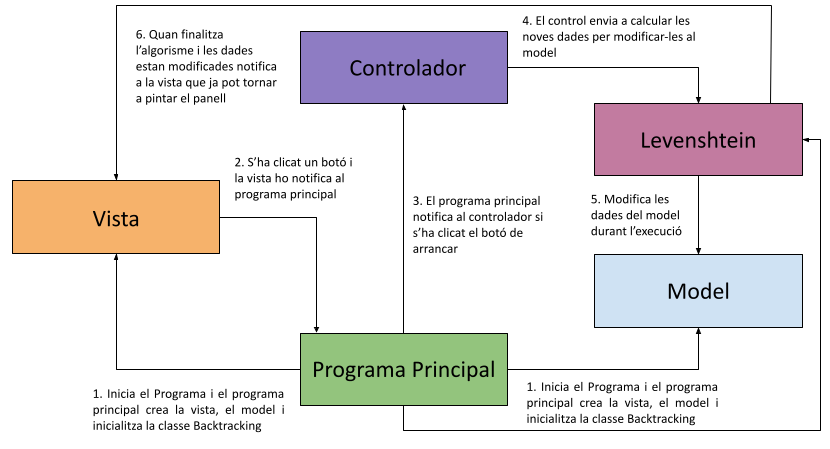
\includegraphics[width=0.388\textwidth]{images/MVC.png}
    \caption{Esquema de com funciona el nostra MVC}
\end{figure}

%3.IMPLEMENTACIÓ DE LA SOLUCIÓ
\section{Implementació de la solució}

\subsection{Problemes a resoldre}
    Durant el desenvolupament d'aquesta pràctica, hem tingut diferents inconvenients/dubtes. Vegeu la llista:

    \begin{itemize}
        \item \textbf{Qualitat de les Dades}: un dels principals problemes que ens varem trobar va ser amb la qualitat de les dades trobades. Molts de diccionaris eren amb formats extranys i depenien del país. En resum, la qualitat de la informació no era gaire bóna.


        \item \textbf{Optimització de l'algoritme}: enteníem la manera d'optimitzar, però no teníem molt clar com ordenar les paraules per longitud, a més d'obtenir els indexos de les localitzacions de les paraules segons la seva longitud.

        \item \textbf{Problema DARRER}: .
        \\
    \end{itemize}
    \subsection{Solucions adoptades}

        \begin{itemize}
            %Redacció arxiu .ltim
            \item \textbf{Manipulació de les Dades}: per a tenir unes dades de qualitat, primer de tot, vàrem haver de canviar la codificació a \textit{UTF-8}.Posteriorment, vàrem convertir tot a minúscules amb l'aplicació \textit{Notepad++}. Això vendria a ser els requisits mínims per a la compatibilitat amb la nostra versió de Java, però hem d'afegir aquests si volem utilitzar l'algoritme optimitzat:

            \begin{itemize}
                \item \textbf{Ordenació per longitud}:

                \item \textbf{Emmagatzematge indexos segons la longitud}:
            \end{itemize}

            Totes aquestes manipulacions s'han aconseguit amb un script de Python, ja que ens resultava més senzill. Vegeu-lo:\\

                %ALGORITME PYTHON
                \begin{algorithm}
                    \caption{Ordenació diccionari i generació metadata}
                    \begin{algorithmic}[1]
                        \State $dicts  \gets llistaNomsDiccionaris$
                        \State $dicts2 \gets llistaNomsDictsOrdenats$\\

                    \For{$\text{dict}$ \textbf{in} $\text{dicts}$}
                                \State $i\gets 0$
                                \For{$\text{word}$ \textbf{in} $\text{dict}$}
                                    \State $words[i]\gets word$
                                    \State $i=i+1$
                                \EndFor
                                \State $sorted\_words \gets words.ordena()$
                                \State $fWrite \gets dict+str(\_sorted.txt)$
                                \State fWrite.write(sorted\_words)
                    \EndFor

                    \\\\

                    \For{$\text{dict}$ \textbf{in} $\text{dicts2}$}
                        \State $indexos \gets \{ \}$
                        \State $pos\gets  0$
                        \State $idx \gets 1$
                        \State $f \gets open(dict)$
                        \State $line \gets dict.readline()$
                        \While{$\text{line}$}
                            \State $\text{lon} \gets \text{len(line) - 1}$
                            \If{$\text{lon} == \text{idx}$}
                                \State $pos \gets pos+1$
                            \Else
                                \State $idx \gets idx+1$
                                \State $indexos[idx]=pos$
                                \State $pos \gets pos+1$
                            \EndIf
                            \State $\text{line} \gets f.\text{readline}()$
                        \EndWhile
                        \State $fitxerOut \gets dict+str(\_metadata.txt)$
                        \State $fitxerOut.write(indexos)$
                    \EndFor
                    \end{algorithmic}
                \end{algorithm}

            En resum el que es fa a l'algoritme de python és el següent:

            \begin{itemize}
                \item \textbf{Lectura de fitxers i ordenació(línies 4-13)}: com podem observar, es van afegint les paraules a un vector i després s'escriu tot a un fitxer, per exemple \textit{CAT\_sorted.txt}, que correspon al català ordenat.\\
                \item \textbf{Lectura de fitxers ordenats i metadata(línies 16-35}: en aquest bucle, el que anam fent és llegir els diccionaris ordenats i mitjançant un diccionari anotam a partir de quina posició comencen les paraules d'aquesta longitud. El diccionari segueix aquest format:
                $$dict=\{x_{0}:y_{0},x_{1}:y_{1},...,x_{n}:y_{n}|x_i \in [L_0,L_n]\}$$

                D'aquesta manera, sabem que $x_i$ pertany al conjunt de longitud possibles de les paraules d'un idioma ($L_i$). Per l'altre lloc $y_i$ correspon a l'índex corresponent on comencen les paraules de $x_i$ longitud.\\ Per exemple: \\

                $$dict=\{1:0,2:24,3:56,...\}$$

                En aquest vector, les paraules amb longitud 3 comencen a la posició 56.
            \end{itemize}

        \end{itemize}


    \subsection{Resolució general}


    %SUBSECCIÓ 3.4
    \subsection{Algoritme de Levenstein}
    \\Per a calcular la distància d'edició entre dues paraules, farem servir l'algorisme de Levenstein. En el nostre programa farem servir, la versió més comú d'aquest algorisme, la versió recursiva.\\

    Les diferentes operacions que es poden aplicar a una paraula per a editar-la son: reemplaçar, esborrarr i insertar.\\
    Tenint aixó en compte, poder realitzar crides recursives en les que modificam la paraula per paràmetre i incrementant el comptador del resultat. Aquest comptador ens indicará la distància resultant entre les dues paraules:
    \begin{itemize}
        \item Afegir: $return  (a_1..a_{n-1}, b_1..b_m) + 1$
        \item Esborrar: $return (a_1..a_n, b_1..b_{m-1}) + 1$
        \item Reemplaçar: $return (a_1..a_{n-1}, b_1..b_{m-1}) + 1$
    \end{itemize}


%MODEL
\section{Model}
 A la classe model tenim diferentes estructures que explicarem més endavant per a poder emmmagatzemar les dades que necesitarem. Aquestes són:
    \begin{verbatim}
    private final String[] dicts;

    private Idioma idioma1;

    private Idioma idioma2;

    public boolean tots;

    private boolean optimitzat;
    \end{verbatim}

    \begin{itemize}
        \item \texttt{dicts}: En aquest array contenim els pseudònims que identifiquen als 10 diferents llenguatges. Aquestes dades ens permeten obtenir totes les diferents opcions a l'hora de comparar un idioma amb tota la resta.\\
        \item \texttt{prog}: Aquesta es una instància de la classe principal.\\
        \item \texttt{idioma1 i idioma2}: Aquestes son les dues diferentes instàncies dels dos idiomes que compararem a l'algorisme, per tant, haurem de establir els valors al model abans de fer l'algorism , ja que lógicament l'algorisme realitza els càlculs sobre els idiomes que es troben al model. Cal dir que quan feim una execució de un idioma amb tota la resta el segon atribut sirà null i no contindrà cap informació, degut a que haurem d'instanciar tota la resta.\\
        \item \texttt{solucionat}: valor booleà que ens indica si ja s'ha trobat la solució, sirem notificats.\\
        \item \texttt{tots}: valor booleà que ens indica si l'usuari vol realitzar una execució d'un idioma amb tota la resta.\\
        \item \texttt{optimitzat}: aquest valor booleà ens indicarà, en aquest cas, si l'usuari desitja executar l'algorsme optimitzat o no, segons si ha marcat la casella a la Vista o no.\\

    \end{itemize}
    Passem ara a explicar els métodes i funcions del Model són principalment \textit{getters i setters}, com per exemple \texttt{getIdioma1();}, que obté el contingut de l'idioma1 que ha seleccionat l'usuari per tal d'obtenir el seu array de paraules i poder executar l'algorisme.
\subsection{Idioma}
La classe Idioma.java emmagatzema les dades individuals d'un diccionari:

    \begin{itemize}
        \item \texttt{List<String> words}: Com el propi nom indica aquest atribut una llista enllaçada de totes les paraules que es troben el fitxer de l'idioma corresponent.
        \item \texttt{List<String> sortedWords}: aquesta es una estructura que conté el contingut de les paraules de l'idioma peró aquest llegeix el fitxer que es troba ordenat.
        \item \texttt{int indexos[]}: Aquest es l'array que conté els indexos de l'array de paraules ordenades on canvia la longitud d'aquestes. Per exemple si les paraules de 3 lletres a l'array de paraules comencen a l'index 30, llavors la tercera posició de l'array d'indexos contindrà el número 30. Aquest array l'inicialitzam llegint dels fitxers continguts a la carpeta metadata. L'utilitat d'aquesta estructura de dades es basa en la facilitat per poder dissenyar l'algorisme optimitzat.
        \item \texttt{String nom}: Com el seu propi nom indica, aquest atribut ens permet obtenir el pseudònim de l'idioma contingut a la classe.


    \end{itemize}
Els mètodes d'aquesta classe son principalment \texttt{getters i setters}. Però, a part d'això, tenim els métodes per inicialitzar les estructures de dades: paraules, paraules ordenades i els indexos.
Els dos primers es basen en la mateixa mecànica de llegir el fitxer seqüencialment amb un bucle while i anara afegint amb el mètode \texttt{.add()}.\\
En canvi, el mètode per inicialitzar l'array de indexos es un poc diferent degut al propi contingut del fitxer. Les línies del fitxer contenen dos valors que ens aporten informació i venen separats per una "," el primer valor numèric que trobam a una línea del fitxer és la longitud en sí de les paraules, mentre que l'altre conté l'index on es comencen a trobar paraules d'aquesta longitud a l'array de paraules. Per fer l'inicialització, a la lectura seqüència hem d'utlitzar el métode \texttt{.split(",")}, a cada nova línea que trobem i guardar els dos valors de l'array que ens retorni el mètode encara que l'únic que ens interesa es l'index que el guardarem a la posició que pertoqui segons la longitud que hagem trobat, d'aquesta manera si l'idioma no té paraules de , per exemple, 14 lletres llavors la posició 14 de l'array d'índexos a la classe \texttt{Idioma}, tindrà un contingut null.

\section{Vista}
La Vista, té com a funció, dintre de l’estructura del programa, mostrar a l’usuari mitjançant un GUI les dades que actualment es troben al model. Els atributs que pertanyen a la
classe principal de la \texttt{Vista} són el següents:
\begin{verbatim}
    private final Main prog;
    private final Panell panell;
    JLabel resultLabel;
    JComboBox<String> comboBox1;
    JComboBox<String> comboBox2;
    JCheckBox checkBox;
\end{verbatim}
\begin{itemize}
    \item \texttt{prog}: atribut que és una instancia del programa principal. Amb ell, podrem obtenir l'atribut \texttt{resultLabel} Aquesta representa la secció de la finestra on mostrarem els resultats obtinguts de l'execució de l'algorisme.\\
    \item \texttt{panell}: atribut que representa l'objecte \texttt{Panell} on dibuixarem tots els punts que generem.\\
    \item \texttt{combobox1 i combobox2}:  aquests son els atributs que contenen els components de selecció múltiple per poder seleccionar els idiomes destí per a realitzar l'algorisme.\\
    \item \texttt{checkBox}: aqui mostram un marcador per si l'usuari desitja aplicar l'opció de l'algorisme optimitzat.
\end{itemize}

Pel que fa als mètodes de la classe simplement són 5:
\begin{verbatim}
    public void mostrar();
    public void initComponents();
    public void actionPerformed(ActionEvent e);
    public void notificar(String s);
    public void mouseClicked(MouseEvent e);
\end{verbatim}
\begin{itemize}
    \item \texttt{mostrar()}: aquest mètode bàsicament crida a totes les funcions encarregades de generar i mostrar les components a pintar\\
    \item \texttt{afegeixComponents()}: en aquesta funció cream els botons, comboboxes i els inicialitzam amb els valors disponibles al programa. També dotam als components d'un LookandFeel per cambiar l'aspecte per defecte. El marcador o checkbox li afegim un ActionListener que modifica l'atribut booleà del model en cas de que l'usuari vulgui realitzar l'opció optimitzada\\
    \item \texttt{actionPerformed(ActionEvent e)} : mètode que s'executa quan algun dels botons de la GUI es clica. Emmagatzema el text que està escrit al botó i l'envia com a comanda al programa principal (que el tenim emmagatzemat a l'atribut \texttt{prog}).\\
    \item \texttt{notificar(String s)}: mètode que utilitzam per notificar al control de que l'usuari ha clicat el botó per a calcular .\\
    \item  \texttt{mouseClicked(MouseEvent e)}: En aquesta funció agafarem els botons seleccionats de model per a que es puguin pintar de manera que es distingueixin de la resta.
\end{itemize}
\\ Els altres mètodes son més simples però igual de rellevants per a la correcta execució del programa. Primer ens trobam dos \texttt{getters}, que ens permeten obtenir l'idioma seleccionat als dos comboboxes i un \texttt{setter}, que ens posibilita editar el Label per mostrar el resultat desde una altre classe.

\subsection{Classe Panell}

%CONTROLADOR
\section{Controlador}

\section{Programa Principal}


%JOCS DE PROVES
\section{Joc de proves}

    \subsection{Primer cas de prova}


    \subsection{Segon cas de prova}

    \subsection{Tercer cas de prova}

\section{Conclusions Finals}




\section{Bibliografia}

    



\end{document}
